\documentclass[11pt,letterpaper]{article}
\usepackage[margin=0.95in]{geometry}
\usepackage[T1]{fontenc}
\usepackage{lmodern}
\usepackage{amsmath,amssymb}
\usepackage{booktabs}
\usepackage{graphicx}
\usepackage{hyperref}
\usepackage{xcolor}
\usepackage{microtype}
\usepackage{tikz}
\usepackage{pgfplots}
\pgfplotsset{compat=1.18}
\usetikzlibrary{arrows.meta,positioning,fit,backgrounds,shapes.geometric}

\hypersetup{
  colorlinks=true,
  linkcolor=blue!60!black,
  citecolor=blue!60!black,
  urlcolor=blue!60!black
}

\title{\textbf{Cost-Aware Hyperparameter Tuning on Local and Enclave Hardware:\\Reference Design, Audit Logging, and Public-Data Benchmark}}

\author{
  Ridwan Salahuddeen\\
  \texttt{ridzy619@yahoo.com}
}

\date{November 2026}

\begin{document}
\maketitle

\begin{abstract}
Organizations subject to data-custody laws or air-gapped security rules often cannot send training data to commercial cloud services. When hyperparameter tuning runs on a fixed local computer instead, repeating early preprocessing and feature-extraction steps takes up most of the available runtime. This note describes a standalone reference design for running memoization- and cost-aware Bayesian optimization (\texttt{eeipu}, version~1.0.0) offline on local hardware or inside a trusted execution environment (TEE), combined with a content-addressed disk cache and a SHA-256 hash-chained audit log. In a benchmark on the public CIFAR-10 dataset with a 120-second compute budget per run on an Apple M1 computer (three random seeds, four methods), \texttt{EEIPU} evaluated $116.0 \pm 21.6$ hyperparameter settings, compared with $41.3 \pm 7.5$ for standard Expected Improvement (\texttt{EI}, $+180.6\%$), $43.3 \pm 3.2$ for \texttt{EI} with Stage~0 caching ($+167.7\%$), and $54.7 \pm 3.2$ for random search ($+112.2\%$). \texttt{EEIPU} reached a mean best validation accuracy of $84.93\% \pm 0.64\%$, compared with $82.33\% \pm 0.99\%$ for \texttt{EI}, $82.27\% \pm 1.29\%$ for \texttt{EI+Cache}, and $82.60\% \pm 0.40\%$ for random search. Stage~0 cache reuse occurred on $78.7\%$ of \texttt{EEIPU} evaluations, used $41.9\%$ less disk space than \texttt{EI+Cache}, added $0.75$~ms per iteration for audit logging, and passed hash-chain verification and tamper checks on all 12 runs.
\end{abstract}

\section{Background and Constraints}
In public safety, healthcare, and defense, legal and institutional rules often require sensitive files to stay on hardware controlled by the organization. In the United States, for example, 18 U.S.C.\ \S\,3509(m) requires child-exploitation evidence to remain in government custody, and the Federal Bureau of Investigation Criminal Justice Information Services (CJIS) Security Policy sets rules for encryption, system isolation, and logging. Similar restrictions apply to patient records under the Health Insurance Portability and Accountability Act (HIPAA).

These rules impose three practical limits on machine learning workflows:
\begin{enumerate}
  \item \textbf{Offline operation:} Hyperparameter search must run locally, either on an on-premises machine or inside a hardware trusted execution environment (TEE), without outbound network traffic or external tracking services.
  \item \textbf{Fixed hardware:} Agencies and laboratories usually work with a fixed workstation or small local server rather than a large cloud cluster, so repeated training runs consume scarce compute time.
  \item \textbf{Record keeping:} When a trained model is used to sort evidence or assist reviewers, examiners need a tamper-evident log linking each trained model and validation score to the exact dataset split, base model, and hyperparameters used.
\end{enumerate}

Many machine learning and multimodal workflows, including vision-transformer key-event detection, speech transcription, and parameter-efficient fine-tuning, are built as multi-stage pipelines. An early stage (Stage~0) prepares data or computes features with a frozen pretrained model, and a later stage (Stage~1) trains a smaller classifier or adapter on those features. Standard Bayesian optimization treats the pipeline as a single black box and re-runs Stage~0 on every trial. Expected Expected Improvement Per Unit Cost (EEIPU)~\cite{essofi2024reducing} addresses this by fitting a separate Gaussian Process cost model for each stage and checking whether reusing cached outputs from earlier stages offers more expected improvement per unit of runtime. This note describes a clean-room local setup for EEIPU with hash-chained logging and reports measurements on a public image dataset.

\section{Reference Design}
The reference code is built from scratch on the open-source \texttt{eeipu} package (version~1.0.0, Apache-2.0 license) using its \texttt{EEIPUOptimizer} ask-and-tell interface. It uses no third-party proprietary code, model weights, or internal vendor designs. Figure~\ref{fig:arch} shows the layout of the local execution boundary and its components.

\begin{figure}[t]
\centering
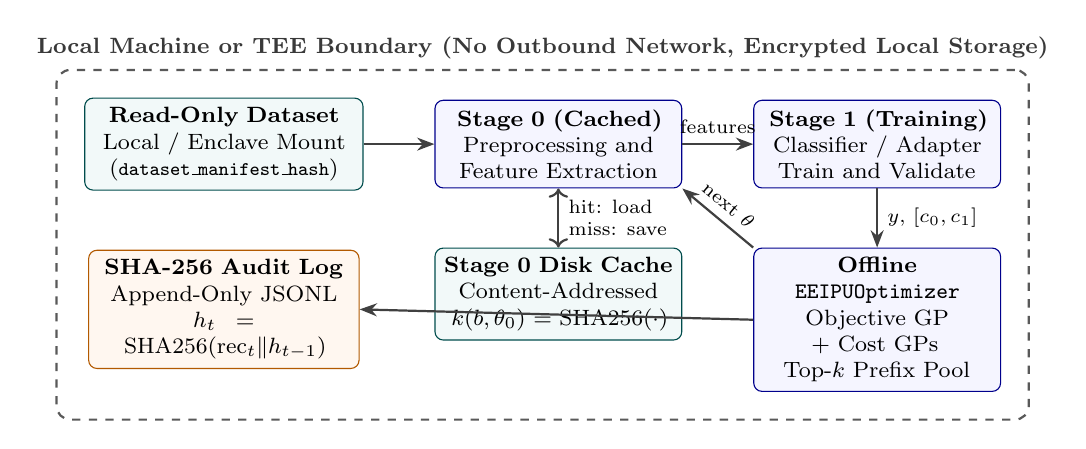
\begin{tikzpicture}[
  node distance=0.65cm and 0.9cm,
  box/.style={rectangle, draw=blue!55!black, fill=blue!4, rounded corners=3pt, minimum height=0.95cm, text width=2.9cm, align=center, font=\footnotesize},
  store/.style={rectangle, draw=teal!60!black, fill=teal!5, rounded corners=3pt, minimum height=0.85cm, text width=2.9cm, align=center, font=\footnotesize},
  audit/.style={rectangle, draw=orange!70!black, fill=orange!6, rounded corners=3pt, minimum height=0.85cm, text width=3.2cm, align=center, font=\footnotesize},
  arrow/.style={-{Stealth[length=2.2mm]}, thick, draw=black!75}
]
  \node[store, text width=3.3cm] (data) {\textbf{Read-Only Dataset}\\Local / Enclave Mount\\(\texttt{\scriptsize dataset\_manifest\_hash})};
  \node[box, right=of data] (stage0) {\textbf{Stage 0 (Cached)}\\Preprocessing and\\Feature Extraction};
  \node[store, below=0.75cm of stage0] (cache) {\textbf{Stage 0 Disk Cache}\\Content-Addressed\\$k(b,\theta_0)=\mathrm{SHA256}(\cdot)$};
  \node[box, right=of stage0] (stage1) {\textbf{Stage 1 (Training)}\\Classifier / Adapter\\Train and Validate};
  \node[box, below=0.75cm of stage1] (opt) {\textbf{Offline \texttt{EEIPUOptimizer}}\\Objective GP + Cost GPs\\Top-$k$ Prefix Pool};
  \node[audit, below=0.75cm of data] (log) {\textbf{SHA-256 Audit Log}\\Append-Only JSONL\\$h_t=\mathrm{SHA256}(\text{rec}_t \| h_{t-1})$};

  \draw[arrow] (data) -- (stage0);
  \draw[arrow] (stage0) -- node[above, font=\scriptsize] {features} (stage1);
  \draw[arrow, <->] (stage0) -- node[right, font=\scriptsize, align=left] {hit: load\\miss: save} (cache);
  \draw[arrow] (stage1) -- node[right, font=\scriptsize, align=left] {$y$, $[c_0, c_1]$} (opt);
  \draw[arrow] (opt.north west) -- node[above, sloped, font=\scriptsize] {next $\theta$} (stage0.south east);
  \draw[arrow] (opt.west) -- (log.east);

  \begin{scope}[on background layer]
    \node[draw=gray!70!black, dashed, thick, rounded corners=5pt, inner sep=10pt,
          fit=(data)(stage0)(cache)(stage1)(opt)(log),
          label={[font=\footnotesize\bfseries, text=gray!45!black]above:Local Machine or TEE Boundary (No Outbound Network, Encrypted Local Storage)}] (boundary) {};
  \end{scope}
\end{tikzpicture}
\caption{Reference layout for offline cost-aware hyperparameter tuning on a local machine or inside a trusted execution environment (TEE). Data, intermediate feature caches, optimization, and audit logs stay inside the execution boundary.}
\label{fig:arch}
\end{figure}

\subsection{Stage Separation and Content-Addressed Caching}
A multi-stage pipeline separates upstream feature extraction (Stage~0) from downstream training (Stage~1). For Stage~0 hyperparameters $\theta_0$ and base-model identifier $b$, the cache key is computed as:
\[
  k(b, \theta_0) = \mathrm{SHA256}\!\left(\mathrm{JSON}_{\text{canonical}}(\{b, \theta_0\})\right)_{[0:16]}.
\]
When a cached file for $k(b, \theta_0)$ already exists on local disk, Stage~0 is skipped and only the file-loading time counts against the wall-clock compute budget. The cached file also records its original uncached Stage~0 runtime. Passing that uncached runtime to the Stage~0 cost Gaussian Process keeps the cost model accurate for uncached settings, while the budget counter tracks actual time spent.

\subsection{Offline Acquisition Loop}
\texttt{EEIPUOptimizer} runs in-process with PyTorch and BoTorch and does not require network access or external experiment trackers (\texttt{wandb} is optional). After $n_{\text{init}}$ independent random warm-up trials drawn across the full search space, each step fits a Gaussian Process to the validation metric $f(\theta)$ and one log-cost Gaussian Process per stage $c_s(\theta_s)$. It then gathers up to $k$ distinct top-scoring Stage~0 prefixes and maximizes the EEIPU acquisition function over both fresh Stage~0 settings and cached prefixes whose Stage~0 cost is discounted to a small constant $\epsilon$.

\subsection{Hash-Chained Audit Log and Enclave Attestation}
After each trial, the runner appends one JSON-Lines (JSONL) entry to an append-only log file. Each entry stores:
\begin{itemize}
  \item \textbf{Provenance fields:} package version (\texttt{eeipu\_version}), base model identifier (\texttt{backbone\_id}), SHA-256 hash of the dataset split manifest (\texttt{dataset\_manifest\_hash}), and SHA-256 hash of the trained Stage~1 model weights (\texttt{model\_weights\_hash}).
  \item \textbf{Run fields:} sequence number (\texttt{seq}), UTC timestamp, method name (\texttt{acq\_type}), random seed, iteration number, hyperparameters, cache-hit flag and key, per-stage runtimes in seconds, and validation accuracy.
  \item \textbf{Hash chain:} the previous entry hash $h_{t-1}$ (starting from 64 zero characters) and the current hash $h_t = \mathrm{SHA256}(\mathrm{JSON}_{\text{canonical}}(\text{record}_t))$.
\end{itemize}
A standalone checker (\texttt{verify\_audit\_log}) recomputes every hash from the first entry to the last entry $h_T$ and reports any change or missing line. On hardware that supports remote attestation (such as AWS Nitro Enclaves, Intel SGX or TDX, or AMD SEV-SNP), placing the final hash $h_T$ in the attestation report's user-data field binds the audit log to the measured enclave image without exporting training data.

\section{Public-Data Benchmark}
To test the design without proprietary code or restricted data, we ran a two-stage image classification benchmark on the public CIFAR-10 dataset. This mirrors the frozen-backbone plus downstream-head structure used in visual triage workflows:
\begin{itemize}
  \item \textbf{Stage~0 (cached):} Resize a CIFAR-10 training subset (\texttt{0\_\_train\_samples} $\in [400, 1600]$) and a fixed $500$-image validation split to \texttt{0\_\_img\_size} $\in [64, 160]$, then extract embeddings with a frozen ImageNet-pretrained ResNet-18 model (\texttt{torchvision.resnet18:IMAGENET1K\_V1}).
  \item \textbf{Stage~1 (trained):} Train a two-layer multilayer perceptron (MLP) with AdamW, tuning learning rate (\texttt{1\_\_lr} $\in [10^{-4}, 10^{-2}]$), weight decay (\texttt{1\_\_weight\_decay} $\in [10^{-5}, 10^{-2}]$), hidden width (\texttt{1\_\_hidden\_dim} $\in [32, 256]$), and epochs (\texttt{1\_\_epochs} $\in [5, 25]$).
  \item \textbf{Compared methods:} Four methods were tested under the same $120$-second wall-clock budget per run ($n_{\text{init}} = 6$, random seeds $\{0, 1, 2\}$): (1)~\texttt{RAND} (uniform random search), (2)~\texttt{EI} (BoTorch \texttt{LogExpectedImprovement} without caching), (3)~\texttt{EI\_CACHE} (\texttt{LogExpectedImprovement} with the same Stage~0 disk cache enabled, to separate passive caching from memoization-aware search), and (4)~\texttt{EEIPU} (memoization-aware search with the Stage~0 disk cache).
  \item \textbf{Hardware:} Personal Apple MacBook Pro (M1), using Apple Metal Performance Shaders (MPS) for ResNet-18 and MLP execution and the CPU for double-precision BoTorch Gaussian Process fitting.
\end{itemize}

\section{Measured Results}
Table~\ref{tab:results} and Figure~\ref{fig:benchmark} show the measured validation accuracy, candidate count, and cache reuse for each method. Table~\ref{tab:overhead} reports measured cache timing, disk usage, and audit-log latency.

\begin{table}[h]
\centering
\footnotesize
\caption{Measured performance under a 120-second wall-clock budget on public CIFAR-10 (mean $\pm$ standard deviation over seeds 0, 1, and 2).}
\label{tab:results}
\begin{tabular}{@{}lcccc@{}}
\toprule
\textbf{Method} & \textbf{Candidates} & \textbf{Best Val.\ Acc.\ (\%)} & \textbf{Stage 0 Hits} & \textbf{Hit Rate} \\
\midrule
Random Search (\texttt{RAND}) & $54.7 \pm 3.2$ & $82.60 \pm 0.40$ & $0.0$ & $0.0\%$ \\
Expected Improvement (\texttt{EI}) & $41.3 \pm 7.5$ & $82.33 \pm 0.99$ & $0.0$ & $0.0\%$ \\
\texttt{EI + Stage 0 Cache} (\texttt{EI\_CACHE}) & $43.3 \pm 3.2$ & $82.27 \pm 1.29$ & $2.7$ & $6.2\%$ \\
\texttt{EEIPU} (this work) & $\mathbf{116.0 \pm 21.6}$ & $\mathbf{84.93 \pm 0.64}$ & $\mathbf{91.3}$ & $\mathbf{78.7\%}$ \\
\bottomrule
\end{tabular}
\end{table}

\begin{figure}[t]
\centering
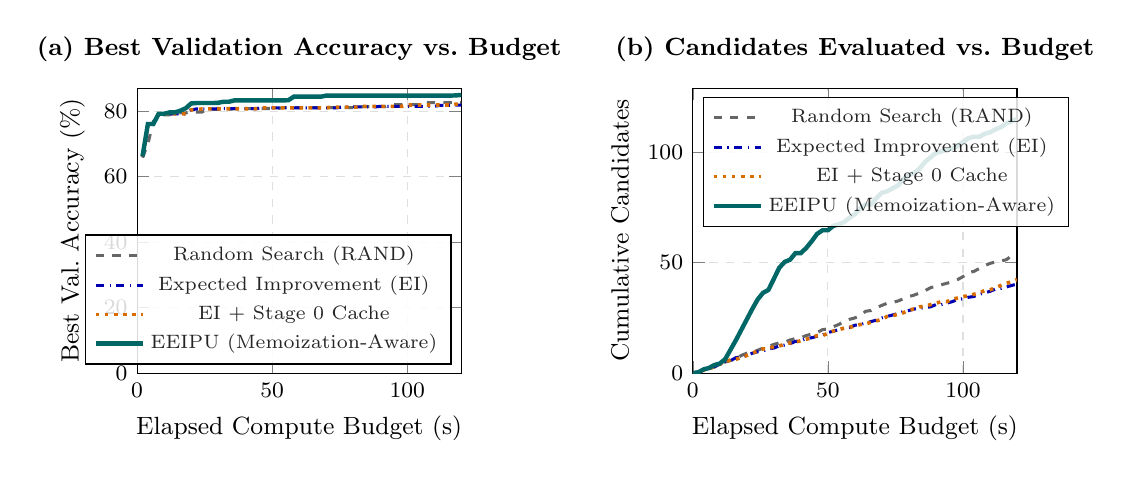
\begin{tikzpicture}
\begin{axis}[
  name=leftplot,
  width=0.47\textwidth,
  height=5.2cm,
  title={(a) Best Validation Accuracy vs.\ Budget},
  xlabel={Elapsed Compute Budget (s)},
  ylabel={Best Val.\ Accuracy (\%)},
  xmin=0, xmax=120,
  ymin=0, ymax=87,
  grid=both,
  grid style={dashed, gray!25},
  legend pos=south east,
  legend style={font=\scriptsize, fill=white, fill opacity=0.85},
  tick label style={font=\footnotesize},
  label style={font=\small},
  title style={font=\small\bfseries}
]
\addplot[color=gray!80!black, dashed, line width=1.1pt] coordinates {(2.00,65.8000) (4.00,70.0000) (6.00,76.8667) (8.00,78.3333) (10.00,78.8667) (12.00,78.8667) (14.00,79.4667) (16.00,79.4667) (18.00,79.4667) (20.00,79.7333) (22.00,79.7333) (24.00,79.7333) (26.00,80.5333) (28.00,80.5333) (30.00,80.5333) (32.00,80.5333) (34.00,80.5333) (36.00,80.7333) (38.00,80.7333) (40.00,80.7333) (42.00,80.7333) (44.00,80.8000) (46.00,80.8000) (48.00,80.8000) (50.00,80.8000) (52.00,80.8000) (54.00,81.0667) (56.00,81.0667) (58.00,81.0667) (60.00,81.0667) (62.00,81.0667) (64.00,81.0667) (66.00,81.0667) (68.00,81.0667) (70.00,81.0667) (72.00,81.0667) (74.00,81.0667) (76.00,81.0667) (78.00,81.0667) (80.00,81.0667) (82.00,81.1333) (84.00,81.4000) (86.00,81.4000) (88.00,81.4000) (90.00,81.4000) (92.00,81.4000) (94.00,82.0000) (96.00,82.0000) (98.00,82.0000) (100.00,82.0000) (102.00,82.0000) (104.00,82.0000) (106.00,82.6000) (108.00,82.6000) (110.00,82.6000) (112.00,82.6000) (114.00,82.6000) (116.00,82.6000) (118.00,82.6000) (120.00,82.6000)};
\addlegendentry{Random Search (RAND)}
\addplot[color=blue!70!black, dashdotted, line width=1.1pt] coordinates {(2.00,66.2000) (4.00,76.0667) (6.00,76.0667) (8.00,79.2000) (10.00,79.2000) (12.00,79.2000) (14.00,79.2000) (16.00,79.2000) (18.00,79.2000) (20.00,80.4000) (22.00,80.6667) (24.00,80.6667) (26.00,80.6667) (28.00,80.6667) (30.00,80.7333) (32.00,80.7333) (34.00,80.7333) (36.00,80.7333) (38.00,80.7333) (40.00,80.7333) (42.00,80.7333) (44.00,80.7333) (46.00,81.0000) (48.00,81.0000) (50.00,81.0000) (52.00,81.0000) (54.00,81.0000) (56.00,81.0000) (58.00,81.0000) (60.00,81.0000) (62.00,81.0000) (64.00,81.0000) (66.00,81.0000) (68.00,81.0000) (70.00,81.0000) (72.00,81.0000) (74.00,81.0000) (76.00,81.2667) (78.00,81.2667) (80.00,81.2667) (82.00,81.2667) (84.00,81.2667) (86.00,81.2667) (88.00,81.2667) (90.00,81.4667) (92.00,81.4667) (94.00,81.4667) (96.00,81.4667) (98.00,81.4667) (100.00,81.4667) (102.00,81.4667) (104.00,81.4667) (106.00,81.4667) (108.00,81.4667) (110.00,81.4667) (112.00,81.7333) (114.00,81.7333) (116.00,81.8000) (118.00,81.8000) (120.00,81.8000)};
\addlegendentry{Expected Improvement (EI)}
\addplot[color=orange!85!black, dotted, line width=1.3pt] coordinates {(2.00,66.2000) (4.00,76.0667) (6.00,76.0667) (8.00,79.2000) (10.00,79.2000) (12.00,79.2000) (14.00,79.2000) (16.00,79.2000) (18.00,79.2000) (20.00,80.4000) (22.00,80.4000) (24.00,80.6667) (26.00,80.6667) (28.00,80.6667) (30.00,80.7333) (32.00,80.7333) (34.00,80.7333) (36.00,80.7333) (38.00,80.7333) (40.00,80.7333) (42.00,80.7333) (44.00,80.7333) (46.00,81.0000) (48.00,81.0000) (50.00,81.0000) (52.00,81.0000) (54.00,81.0000) (56.00,81.0000) (58.00,81.0000) (60.00,81.0000) (62.00,81.0000) (64.00,81.0000) (66.00,81.0000) (68.00,81.0000) (70.00,81.0000) (72.00,81.2000) (74.00,81.2000) (76.00,81.2000) (78.00,81.2000) (80.00,81.2000) (82.00,81.2000) (84.00,81.4667) (86.00,81.4667) (88.00,81.4667) (90.00,81.4667) (92.00,81.4667) (94.00,81.4667) (96.00,81.4667) (98.00,81.4667) (100.00,81.8667) (102.00,81.8667) (104.00,81.8667) (106.00,81.8667) (108.00,81.8667) (110.00,81.8667) (112.00,81.8667) (114.00,81.8667) (116.00,81.8667) (118.00,82.1333) (120.00,82.2000)};
\addlegendentry{EI + Stage 0 Cache}
\addplot[color=teal!80!black, solid, line width=1.6pt] coordinates {(2.00,66.2000) (4.00,76.0667) (6.00,76.0667) (8.00,79.2000) (10.00,79.2000) (12.00,79.6000) (14.00,79.6000) (16.00,80.1333) (18.00,80.8667) (20.00,82.3333) (22.00,82.4667) (24.00,82.4667) (26.00,82.4667) (28.00,82.4667) (30.00,82.5333) (32.00,82.8667) (34.00,82.8667) (36.00,83.2667) (38.00,83.2667) (40.00,83.2667) (42.00,83.2667) (44.00,83.2667) (46.00,83.2667) (48.00,83.2667) (50.00,83.2667) (52.00,83.2667) (54.00,83.2667) (56.00,83.3333) (58.00,84.4000) (60.00,84.4000) (62.00,84.4000) (64.00,84.4000) (66.00,84.4000) (68.00,84.4000) (70.00,84.7333) (72.00,84.7333) (74.00,84.7333) (76.00,84.7333) (78.00,84.7333) (80.00,84.7333) (82.00,84.7333) (84.00,84.7333) (86.00,84.7333) (88.00,84.7333) (90.00,84.7333) (92.00,84.7333) (94.00,84.7333) (96.00,84.7333) (98.00,84.7333) (100.00,84.7333) (102.00,84.7333) (104.00,84.7333) (106.00,84.7333) (108.00,84.7333) (110.00,84.7333) (112.00,84.7333) (114.00,84.7333) (116.00,84.7333) (118.00,84.8000) (120.00,84.9333)};
\addlegendentry{EEIPU (Memoization-Aware)}
\end{axis}
\begin{axis}[
  at={(leftplot.outer east)},
  anchor=outer west,
  xshift=0.4cm,
  width=0.47\textwidth,
  height=5.2cm,
  title={(b) Candidates Evaluated vs.\ Budget},
  xlabel={Elapsed Compute Budget (s)},
  ylabel={Cumulative Candidates},
  xmin=0, xmax=120,
  ymin=0, ymax=129,
  grid=both,
  grid style={dashed, gray!25},
  legend pos=north west,
  legend style={font=\scriptsize, fill=white, fill opacity=0.85},
  tick label style={font=\footnotesize},
  label style={font=\small},
  title style={font=\small\bfseries}
]
\addplot[color=gray!80!black, dashed, line width=1.1pt] coordinates {(0.00,0.0000) (2.00,0.6667) (4.00,1.0000) (6.00,2.0000) (8.00,2.6667) (10.00,4.0000) (12.00,5.0000) (14.00,5.6667) (16.00,6.6667) (18.00,8.0000) (20.00,9.0000) (22.00,9.3333) (24.00,10.3333) (26.00,11.3333) (28.00,12.0000) (30.00,13.0000) (32.00,13.6667) (34.00,14.0000) (36.00,15.0000) (38.00,15.6667) (40.00,16.0000) (42.00,17.0000) (44.00,17.6667) (46.00,18.3333) (48.00,19.6667) (50.00,20.0000) (52.00,21.0000) (54.00,22.0000) (56.00,23.3333) (58.00,24.3333) (60.00,25.0000) (62.00,26.0000) (64.00,28.0000) (66.00,28.3333) (68.00,29.6667) (70.00,30.6667) (72.00,31.6667) (74.00,32.0000) (76.00,32.6667) (78.00,33.6667) (80.00,34.6667) (82.00,35.3333) (84.00,36.3333) (86.00,37.3333) (88.00,38.6667) (90.00,39.3333) (92.00,40.0000) (94.00,40.6667) (96.00,41.3333) (98.00,42.3333) (100.00,43.6667) (102.00,45.6667) (104.00,46.0000) (106.00,47.3333) (108.00,48.6667) (110.00,49.6667) (112.00,50.3333) (114.00,50.6667) (116.00,51.3333) (118.00,53.0000) (120.00,53.6667)};
\addlegendentry{Random Search (RAND)}
\addplot[color=blue!70!black, dashdotted, line width=1.1pt] coordinates {(0.00,0.0000) (2.00,0.3333) (4.00,1.3333) (6.00,2.0000) (8.00,3.0000) (10.00,4.0000) (12.00,5.3333) (14.00,5.6667) (16.00,7.0000) (18.00,7.3333) (20.00,8.0000) (22.00,9.0000) (24.00,9.6667) (26.00,10.0000) (28.00,11.0000) (30.00,11.3333) (32.00,12.3333) (34.00,12.6667) (36.00,13.3333) (38.00,14.3333) (40.00,14.6667) (42.00,15.6667) (44.00,16.0000) (46.00,16.6667) (48.00,17.3333) (50.00,18.3333) (52.00,19.0000) (54.00,19.6667) (56.00,20.3333) (58.00,20.6667) (60.00,21.6667) (62.00,22.0000) (64.00,22.6667) (66.00,23.3333) (68.00,24.0000) (70.00,25.0000) (72.00,25.6667) (74.00,26.3333) (76.00,27.0000) (78.00,28.0000) (80.00,28.3333) (82.00,29.0000) (84.00,29.3333) (86.00,29.6667) (88.00,30.0000) (90.00,31.0000) (92.00,31.0000) (94.00,31.6667) (96.00,32.3333) (98.00,33.3333) (100.00,33.6667) (102.00,34.3333) (104.00,34.6667) (106.00,35.6667) (108.00,36.3333) (110.00,37.0000) (112.00,38.0000) (114.00,38.3333) (116.00,39.0000) (118.00,39.6667) (120.00,40.3333)};
\addlegendentry{Expected Improvement (EI)}
\addplot[color=orange!85!black, dotted, line width=1.3pt] coordinates {(0.00,0.0000) (2.00,0.3333) (4.00,1.3333) (6.00,2.0000) (8.00,3.0000) (10.00,4.0000) (12.00,5.0000) (14.00,6.0000) (16.00,6.3333) (18.00,7.0000) (20.00,8.0000) (22.00,9.0000) (24.00,10.0000) (26.00,11.0000) (28.00,11.0000) (30.00,12.0000) (32.00,12.3333) (34.00,13.0000) (36.00,13.6667) (38.00,14.0000) (40.00,14.6667) (42.00,15.3333) (44.00,16.0000) (46.00,17.0000) (48.00,17.0000) (50.00,18.0000) (52.00,19.0000) (54.00,19.6667) (56.00,20.3333) (58.00,20.6667) (60.00,21.3333) (62.00,22.0000) (64.00,22.3333) (66.00,23.0000) (68.00,23.6667) (70.00,24.3333) (72.00,25.6667) (74.00,26.0000) (76.00,26.6667) (78.00,27.3333) (80.00,28.6667) (82.00,29.0000) (84.00,30.0000) (86.00,30.3333) (88.00,31.0000) (90.00,31.6667) (92.00,32.3333) (94.00,32.3333) (96.00,33.3333) (98.00,34.0000) (100.00,34.6667) (102.00,35.0000) (104.00,35.6667) (106.00,36.3333) (108.00,37.3333) (110.00,37.6667) (112.00,38.6667) (114.00,39.6667) (116.00,40.6667) (118.00,41.3333) (120.00,42.3333)};
\addlegendentry{EI + Stage 0 Cache}
\addplot[color=teal!80!black, solid, line width=1.6pt] coordinates {(0.00,0.0000) (2.00,0.3333) (4.00,1.6667) (6.00,2.3333) (8.00,3.6667) (10.00,4.3333) (12.00,6.3333) (14.00,10.6667) (16.00,15.0000) (18.00,19.6667) (20.00,24.3333) (22.00,29.0000) (24.00,33.3333) (26.00,36.3333) (28.00,37.6667) (30.00,42.6667) (32.00,47.6667) (34.00,50.3333) (36.00,51.3333) (38.00,54.3333) (40.00,54.3333) (42.00,56.6667) (44.00,59.6667) (46.00,63.0000) (48.00,64.6667) (50.00,64.6667) (52.00,66.6667) (54.00,67.3333) (56.00,68.3333) (58.00,70.3333) (60.00,72.0000) (62.00,74.6667) (64.00,76.3333) (66.00,76.3333) (68.00,79.3333) (70.00,81.6667) (72.00,82.3333) (74.00,83.6667) (76.00,85.0000) (78.00,88.0000) (80.00,89.6667) (82.00,90.6667) (84.00,92.6667) (86.00,95.6667) (88.00,97.6667) (90.00,99.6667) (92.00,100.3333) (94.00,101.0000) (96.00,101.6667) (98.00,102.6667) (100.00,104.6667) (102.00,106.3333) (104.00,107.0000) (106.00,107.0000) (108.00,108.3333) (110.00,109.0000) (112.00,110.3333) (114.00,111.3333) (116.00,113.0000) (118.00,114.0000) (120.00,115.0000)};
\addlegendentry{EEIPU (Memoization-Aware)}
\end{axis}
\end{tikzpicture}
\caption{Mean validation accuracy and cumulative candidate throughput across seeds versus elapsed compute budget on public CIFAR-10 (Apple M1).}
\label{fig:benchmark}
\end{figure}


\begin{table}[h]
\centering
\footnotesize
\caption{Measured cache timing, disk usage, and audit-log latency (means over seeds 0, 1, and 2).}
\label{tab:overhead}
\begin{tabular}{@{}lccccc@{}}
\toprule
\textbf{Method} & \textbf{Stage 0 Miss (s)} & \textbf{Stage 0 Hit (ms)} & \textbf{Cache (MB)} & \textbf{Audit Write (ms)} & \textbf{Verify (ms)} \\
\midrule
\texttt{RAND} & $1.706$ & --- & $0.0$ & $0.58$ & $2.64$ \\
\texttt{EI} & $2.542$ & --- & $0.0$ & $0.67$ & $2.28$ \\
\texttt{EI\_CACHE} & $2.571$ & $5.89$ & $128.8$ & $0.66$ & $1.44$ \\
\texttt{EEIPU} & $2.514$ & $\mathbf{2.81}$ & $\mathbf{74.8}$ & $0.75$ & $4.24$ \\
\bottomrule
\end{tabular}
\end{table}

The measurements show four main patterns:
\begin{enumerate}
  \item \textbf{More evaluations and higher accuracy:} Within the 120-second budget, \texttt{EEIPU} evaluated $116.0 \pm 21.6$ candidates, which is $+180.6\%$ more than \texttt{EI} ($41.3 \pm 7.5$), $+167.7\%$ more than \texttt{EI\_CACHE} ($43.3 \pm 3.2$), and $+112.2\%$ more than \texttt{RAND} ($54.7 \pm 3.2$). \texttt{EEIPU} also reached the highest validation accuracy on each of the three seeds ($84.2\%$, $85.2\%$, and $85.4\%$; mean $84.93\% \pm 0.64\%$), exceeding \texttt{EI} by $2.60$ percentage points, \texttt{EI\_CACHE} by $2.67$ percentage points, and \texttt{RAND} by $2.33$ percentage points.
  \item \textbf{Effect of passive caching alone:} Giving standard \texttt{EI} the same Stage~0 disk cache (\texttt{EI\_CACHE}) produced an average of only $2.7$ cache hits ($6.2\%$ hit rate) and $2.0$ additional candidates, because continuous acquisition rarely selects an identical Stage~0 setting twice. \texttt{EI\_CACHE} also wrote $128.8$~MB of cached files per run, whereas \texttt{EEIPU} achieved a $78.7\%$ hit rate using $74.8$~MB ($41.9\%$ less disk space) by reusing a smaller set of high-scoring Stage~0 prefixes.
  \item \textbf{Cache read speed:} Loading cached Stage~0 features took $2.81$~ms on average, compared with $2.514$~s to compute Stage~0 from scratch (an $895\times$ reduction in Stage~0 time on a cache hit).
  \item \textbf{Audit-log cost and tamper checks:} Writing each SHA-256 log record took $0.58$ to $0.75$~ms per iteration (less than $0.05\%$ of an uncached evaluation), and checking a complete trial log took $1.44$ to $4.24$~ms. All 12 logs ($4$ methods $\times$ $3$ seeds) passed \texttt{verify\_audit\_log}. In an automated tamper test (\texttt{verify\_tamper\_detection}) that modified a single recorded accuracy value in a copy of each log, the checker flagged all 12 modified logs ($100\%$).
\end{enumerate}

\section{Scope, Limitations, and Future Work}
This work is a clean-room reference implementation tested only on public data (CIFAR-10) using personal Apple M1 hardware. It does not report measurements inside a hardware TEE; instead, it documents the offline execution layout, content-addressed cache, and hash-chained log format needed for local and enclave deployment. Planned follow-up work includes testing Vision Transformer (\texttt{vit\_b\_16}, already implemented in \texttt{pipeline.py}), speech-transcription, and parameter-efficient fine-tuning pipelines on public datasets, as well as adding container templates that bind the terminal audit hash $h_T$ to hardware TEE attestation quotes.

\section{Reproducibility and Code Availability}
The benchmark scripts, audit-log verifier, and \texttt{eeipu} package (version~1.0.0, Apache-2.0 license) are available in the \texttt{benchmarks/on\_prem\_enclave/} directory of \url{https://github.com/ridwan-salau/cost-aware-bo}. All results were generated with Python~3.12, PyTorch~2.15, and BoTorch~0.18 using:
\begin{verbatim}
python run_benchmark.py --budget-sec 120 --n-init 6 --seeds 0 1 2
python plot_results.py --results-dir ./results --budget-sec 120
\end{verbatim}

\begin{thebibliography}{1}
\bibitem{essofi2024reducing}
A.~Essofi, R.~Salahuddeen, M.~Nwadike, E.~Zhalieva, K.~Zhang, E.~P. Xing, W.~Neiswanger, and Q.~Ho,
``Reducing hyperparameter tuning costs in ML, vision and language model training pipelines via memoization-awareness,''
\emph{arXiv preprint arXiv:2411.03731}, 2024.
\end{thebibliography}

\end{document}
